% Options for packages loaded elsewhere
\PassOptionsToPackage{unicode}{hyperref}
\PassOptionsToPackage{hyphens}{url}
\PassOptionsToPackage{dvipsnames,svgnames,x11names}{xcolor}
%
\documentclass[
]{article}
\usepackage{amsmath,amssymb}
\usepackage{lmodern}
\usepackage{iftex}
\ifPDFTeX
  \usepackage[T1]{fontenc}
  \usepackage[utf8]{inputenc}
  \usepackage{textcomp} % provide euro and other symbols
\else % if luatex or xetex
  \usepackage{unicode-math}
  \defaultfontfeatures{Scale=MatchLowercase}
  \defaultfontfeatures[\rmfamily]{Ligatures=TeX,Scale=1}
\fi
% Use upquote if available, for straight quotes in verbatim environments
\IfFileExists{upquote.sty}{\usepackage{upquote}}{}
\IfFileExists{microtype.sty}{% use microtype if available
  \usepackage[]{microtype}
  \UseMicrotypeSet[protrusion]{basicmath} % disable protrusion for tt fonts
}{}
\makeatletter
\@ifundefined{KOMAClassName}{% if non-KOMA class
  \IfFileExists{parskip.sty}{%
    \usepackage{parskip}
  }{% else
    \setlength{\parindent}{0pt}
    \setlength{\parskip}{6pt plus 2pt minus 1pt}}
}{% if KOMA class
  \KOMAoptions{parskip=half}}
\makeatother
\usepackage{xcolor}
\usepackage[margin=1in]{geometry}
\usepackage{color}
\usepackage{fancyvrb}
\newcommand{\VerbBar}{|}
\newcommand{\VERB}{\Verb[commandchars=\\\{\}]}
\DefineVerbatimEnvironment{Highlighting}{Verbatim}{commandchars=\\\{\}}
% Add ',fontsize=\small' for more characters per line
\usepackage{framed}
\definecolor{shadecolor}{RGB}{248,248,248}
\newenvironment{Shaded}{\begin{snugshade}}{\end{snugshade}}
\newcommand{\AlertTok}[1]{\textcolor[rgb]{0.94,0.16,0.16}{#1}}
\newcommand{\AnnotationTok}[1]{\textcolor[rgb]{0.56,0.35,0.01}{\textbf{\textit{#1}}}}
\newcommand{\AttributeTok}[1]{\textcolor[rgb]{0.77,0.63,0.00}{#1}}
\newcommand{\BaseNTok}[1]{\textcolor[rgb]{0.00,0.00,0.81}{#1}}
\newcommand{\BuiltInTok}[1]{#1}
\newcommand{\CharTok}[1]{\textcolor[rgb]{0.31,0.60,0.02}{#1}}
\newcommand{\CommentTok}[1]{\textcolor[rgb]{0.56,0.35,0.01}{\textit{#1}}}
\newcommand{\CommentVarTok}[1]{\textcolor[rgb]{0.56,0.35,0.01}{\textbf{\textit{#1}}}}
\newcommand{\ConstantTok}[1]{\textcolor[rgb]{0.00,0.00,0.00}{#1}}
\newcommand{\ControlFlowTok}[1]{\textcolor[rgb]{0.13,0.29,0.53}{\textbf{#1}}}
\newcommand{\DataTypeTok}[1]{\textcolor[rgb]{0.13,0.29,0.53}{#1}}
\newcommand{\DecValTok}[1]{\textcolor[rgb]{0.00,0.00,0.81}{#1}}
\newcommand{\DocumentationTok}[1]{\textcolor[rgb]{0.56,0.35,0.01}{\textbf{\textit{#1}}}}
\newcommand{\ErrorTok}[1]{\textcolor[rgb]{0.64,0.00,0.00}{\textbf{#1}}}
\newcommand{\ExtensionTok}[1]{#1}
\newcommand{\FloatTok}[1]{\textcolor[rgb]{0.00,0.00,0.81}{#1}}
\newcommand{\FunctionTok}[1]{\textcolor[rgb]{0.00,0.00,0.00}{#1}}
\newcommand{\ImportTok}[1]{#1}
\newcommand{\InformationTok}[1]{\textcolor[rgb]{0.56,0.35,0.01}{\textbf{\textit{#1}}}}
\newcommand{\KeywordTok}[1]{\textcolor[rgb]{0.13,0.29,0.53}{\textbf{#1}}}
\newcommand{\NormalTok}[1]{#1}
\newcommand{\OperatorTok}[1]{\textcolor[rgb]{0.81,0.36,0.00}{\textbf{#1}}}
\newcommand{\OtherTok}[1]{\textcolor[rgb]{0.56,0.35,0.01}{#1}}
\newcommand{\PreprocessorTok}[1]{\textcolor[rgb]{0.56,0.35,0.01}{\textit{#1}}}
\newcommand{\RegionMarkerTok}[1]{#1}
\newcommand{\SpecialCharTok}[1]{\textcolor[rgb]{0.00,0.00,0.00}{#1}}
\newcommand{\SpecialStringTok}[1]{\textcolor[rgb]{0.31,0.60,0.02}{#1}}
\newcommand{\StringTok}[1]{\textcolor[rgb]{0.31,0.60,0.02}{#1}}
\newcommand{\VariableTok}[1]{\textcolor[rgb]{0.00,0.00,0.00}{#1}}
\newcommand{\VerbatimStringTok}[1]{\textcolor[rgb]{0.31,0.60,0.02}{#1}}
\newcommand{\WarningTok}[1]{\textcolor[rgb]{0.56,0.35,0.01}{\textbf{\textit{#1}}}}
\usepackage{graphicx}
\makeatletter
\def\maxwidth{\ifdim\Gin@nat@width>\linewidth\linewidth\else\Gin@nat@width\fi}
\def\maxheight{\ifdim\Gin@nat@height>\textheight\textheight\else\Gin@nat@height\fi}
\makeatother
% Scale images if necessary, so that they will not overflow the page
% margins by default, and it is still possible to overwrite the defaults
% using explicit options in \includegraphics[width, height, ...]{}
\setkeys{Gin}{width=\maxwidth,height=\maxheight,keepaspectratio}
% Set default figure placement to htbp
\makeatletter
\def\fps@figure{htbp}
\makeatother
\setlength{\emergencystretch}{3em} % prevent overfull lines
\providecommand{\tightlist}{%
  \setlength{\itemsep}{0pt}\setlength{\parskip}{0pt}}
\setcounter{secnumdepth}{-\maxdimen} % remove section numbering
\usepackage{multirow}
%\PassOptionsToPackage{table,xcdraw}{xcolor}
%\usepackage[usenames,dvipsnames]{xcolor}
\usepackage{colortbl}
\usepackage{makecell}
%\usepackage[spanish,es-nolists]{babel}
%%\usepackage[spanish]{babel}
%% change fontsize of R code
%%colorines
%\usepackage{amsmath,color,array,booktabs,algorithm2e}
%\newcommand\blue[1]{\textcolor{blue}{#1}}
%\newcommand\red[1]{\textcolor{red}{#1}}

%% change fontsize of output
%\let\oldverbatim\verbatim
%\let\endoldverbatim\endverbatim
%\renewenvironment{verbatim}{\scriptsize\oldverbatim}{\endoldverbatim}
%\usepackage{multirow}
%\PassOptionsToPackage{table,xcdraw}{xcolor}
%\usepackage[table,xcdraw]{xcolor}
%\usepackage{colortbl}

\usepackage{makecell}
 \usepackage{booktabs}
 \usepackage{adjustbox}
 \usepackage{amsmath,color,array,booktabs,algorithm2e}
 \definecolor{LightBlue}{RGB}{173,216,230}
 \newcommand\blue[1]{\textcolor{blue}{#1}}
 \newcommand\red[1]{\textcolor{red}{#1}}
 %\setbeamertemplate{navigation symbols}{}
 %\setbeamertemplate{footline}[page number]
 \usepackage{mathdots}
\usepackage{yhmath}
\usepackage{mathdots}
\usepackage{MnSymbol}
\renewcommand{\contentsname}{Índice}
%\renewcommand{\chaptername}{Parte}
%\renewcommand{\sectionname}{Lección}
%%%%%%%%%%

%\usepackage[spanish,es-nolists]{babel}
%%\usepackage[spanish]{babel}
%% change fontsize of R code
%%colorines
%\usepackage{amsmath,color,array,booktabs,algorithm2e}
%\newcommand\blue[1]{\textcolor{blue}{#1}}
%\newcommand\red[1]{\textcolor{red}{#1}}

%% change fontsize of output
%\let\oldverbatim\verbatim
%\let\endoldverbatim\endverbatim
%\renewenvironment{verbatim}{\tiny\oldverbatim}{\endoldverbatim}
%\usepackage[table,xcdraw]{xcolor}

\ifLuaTeX
  \usepackage{selnolig}  % disable illegal ligatures
\fi
\IfFileExists{bookmark.sty}{\usepackage{bookmark}}{\usepackage{hyperref}}
\IfFileExists{xurl.sty}{\usepackage{xurl}}{} % add URL line breaks if available
\urlstyle{same} % disable monospaced font for URLs
\hypersetup{
  pdftitle={Taller 2 en grupo 1.5 puntos nota final},
  pdfauthor={Estadística},
  colorlinks=true,
  linkcolor={Maroon},
  filecolor={Maroon},
  citecolor={Blue},
  urlcolor={Blue},
  pdfcreator={LaTeX via pandoc}}

\title{Taller 2 en grupo 1.5 puntos nota final}
\author{Estadística}
\date{02 enero, 2023}

\begin{document}
\maketitle

{
\hypersetup{linkcolor=blue}
\setcounter{tocdepth}{3}
\tableofcontents
}
Nombre del grupo: Grupo NOMBRE

Autores

\begin{enumerate}
\def\labelenumi{\arabic{enumi}.}
\tightlist
\item
  Apellidos, Nombre
\item
  Apellidos, Nombre
\item
  Apellidos, Nombre
\item
  Apellidos, Nombre
\item
  Apellidos, Nombre
\end{enumerate}

\textbf{INSTRUCCIONES}

Comentarios:

\begin{itemize}
\item
  Para hacer los cálculos solicitados en los apartados anterior se deben
  eliminar los valores no disponibles (\texttt{NA}) de las variables.
\item
  Siempre que sea posible se deben utilizar las funciones de R
  explicadas en clase para resolver los ejercicios.
\item
  Debe redactar un documento utilizando Rmarkdown con las respuestas a
  estas preguntas y que incluya el código R utilizado. También debe
  generar (Knit) una versión HTML del documento.
\end{itemize}

El documento, en formato .Rmd y .html o .pdf , se debe \textbf{entregar
a Aula Digital antes del 22 de diciembre}.

\hypertarget{parte-1.-descripciuxf3n-de-datos-tidyverse}{%
\section{Parte 1. Descripción de datos
tidyverse}\label{parte-1.-descripciuxf3n-de-datos-tidyverse}}

Considera el conjunto de datos \texttt{examenes.csv} que contiene las
siguientes variables:

\begin{itemize}
\item
  \texttt{gender}: sexo del estudiante masculino (``male'') o femenino
  (``female'').
\item
  \texttt{race/ethnicity}: raza del estudiante (grupos desde el A hasta
  el E).
\item
  \texttt{parental\ level\ of\ education}: nivel educativo de los padres
  desde algo de estudios secundarios (``some high school'') hasta master
  (``master degree'').
\item
  \texttt{lunch}: tipo de precio que paga el estudiante por la comida
  que recibe en el centro educativo: normal (``standard'') o con
  descuento (``free/reduced'').
\item
  \texttt{test\ preparation\ course}: si el estudiante ha tomado un
  curso de preparación para el examen de acceso a la Universidad, dos
  posibles valores: lo completó (``completed''), no lo tomó (``none'').
\item
  \texttt{math\ score}: nota que obtuvo el estudiante en la parte de
  matemáticas del examen de acceso a la Universidad. Valores del 0 al
  100, donde el 100 es la máxima puntuación.
\item
  \texttt{reading\ score}: nota que obtuvo el estudiante en la parte de
  lectura del examen de acceso a la Universidad. Valores del 0 al 100,
  donde el 100 es la máxima puntuación.
\item
  \texttt{writing\ score}: nota que obtuvo el estudiante en la parte de
  redacción del examen de acceso a la Universidad. Valores del 0 al 100,
  donde el 100 es la máxima puntuación.
\end{itemize}

A continuación te presento la estructura del conjunto de datos:

\begin{Shaded}
\begin{Highlighting}[]
\FunctionTok{library}\NormalTok{(readr)}
\NormalTok{datos }\OtherTok{\textless{}{-}} \FunctionTok{read\_csv}\NormalTok{(}\StringTok{"data/examenes.csv"}\NormalTok{)}
\FunctionTok{library}\NormalTok{(tidyverse)}
\FunctionTok{glimpse}\NormalTok{(datos)}
\end{Highlighting}
\end{Shaded}

\begin{verbatim}
## Rows: 1,000
## Columns: 8
## $ gender                        <chr> "male", "female", "male", "male", "male"~
## $ `race/ethnicity`              <chr> "group A", "group D", "group E", "group ~
## $ `parental level of education` <chr> "high school", "some high school", "some~
## $ lunch                         <chr> "standard", "free/reduced", "free/reduce~
## $ `test preparation course`     <chr> "completed", "none", "none", "none", "co~
## $ `math score`                  <dbl> 67, 40, 59, 77, 78, 63, 62, 93, 63, 47, ~
## $ `reading score`               <dbl> 67, 59, 60, 78, 73, 77, 59, 88, 56, 42, ~
## $ `writing score`               <dbl> 63, 55, 50, 68, 68, 76, 63, 84, 65, 45, ~
\end{verbatim}

\hypertarget{cuestiuxf3n-1.-1-punto}{%
\subsection{\texorpdfstring{Cuestión 1. \textbf{1
punto}}{Cuestión 1. 1 punto}}\label{cuestiuxf3n-1.-1-punto}}

\begin{enumerate}
\def\labelenumi{\alph{enumi}.}
\tightlist
\item
  Describe lo que se calcula con el siguiente código
\end{enumerate}

\begin{Shaded}
\begin{Highlighting}[]
\NormalTok{datos }\OtherTok{\textless{}{-}} \FunctionTok{drop\_na}\NormalTok{(datos)}
\NormalTok{datos }\SpecialCharTok{\%\textgreater{}\%} \FunctionTok{group\_by}\NormalTok{(gender)}\SpecialCharTok{\%\textgreater{}\%}
  \FunctionTok{summarise}\NormalTok{(}\AttributeTok{frecuencia=}\FunctionTok{length}\NormalTok{(gender))}\SpecialCharTok{\%\textgreater{}\%}
  \FunctionTok{mutate}\NormalTok{(}\AttributeTok{porcentaje=}\NormalTok{frecuencia}\SpecialCharTok{/}\FunctionTok{sum}\NormalTok{(frecuencia)}\SpecialCharTok{*}\DecValTok{100}\NormalTok{)}
\NormalTok{df}\OtherTok{\textless{}{-}}\NormalTok{ datos }\SpecialCharTok{\%\textgreater{}\%} \FunctionTok{group\_by}\NormalTok{(}\StringTok{\textasciigrave{}}\AttributeTok{race/ethnicity}\StringTok{\textasciigrave{}}\NormalTok{) }\SpecialCharTok{\%\textgreater{}\%}
 \FunctionTok{summarise}\NormalTok{(}\AttributeTok{frecuencia=}\FunctionTok{length}\NormalTok{(}\StringTok{\textasciigrave{}}\AttributeTok{race/ethnicity}\StringTok{\textasciigrave{}}\NormalTok{)) }\SpecialCharTok{\%\textgreater{}\%}
 \FunctionTok{arrange}\NormalTok{(}\FunctionTok{desc}\NormalTok{(frecuencia)) }
\NormalTok{df}
\end{Highlighting}
\end{Shaded}

\begin{enumerate}
\def\labelenumi{\alph{enumi}.}
\setcounter{enumi}{1}
\tightlist
\item
  Da el código de ggplot2 que genera este gráfico. Comenta los
  resultados
\end{enumerate}

\begin{center}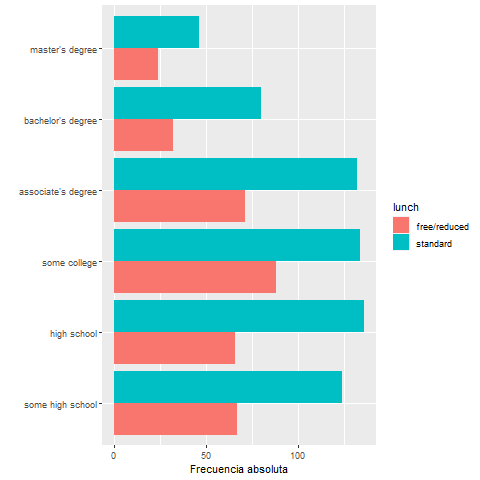
\includegraphics[width=0.6\linewidth]{plot1} \end{center}

\hypertarget{cuestiuxf3n-2.-1-punto}{%
\subsection{\texorpdfstring{Cuestión 2. \textbf{1
punto}}{Cuestión 2. 1 punto}}\label{cuestiuxf3n-2.-1-punto}}

Explica lo que se obtiene en la tibble \texttt{df2} y dibuja y analiza
el gráfico que se genera en el contexto del problema.

\begin{Shaded}
\begin{Highlighting}[]
\NormalTok{df2}\OtherTok{\textless{}{-}}\NormalTok{ datos }\SpecialCharTok{\%\textgreater{}\%}
\NormalTok{  tidyr}\SpecialCharTok{::}\FunctionTok{pivot\_longer}\NormalTok{(}
    \AttributeTok{cols=}\FunctionTok{contains}\NormalTok{(}\StringTok{"score"}\NormalTok{),}
    \AttributeTok{names\_to=}\StringTok{"area"}\NormalTok{, }\AttributeTok{values\_to=}\StringTok{"notas"}\NormalTok{) }\SpecialCharTok{\%\textgreater{}\%}
  \FunctionTok{select}\NormalTok{(}\StringTok{"area"}\NormalTok{, }\StringTok{\textasciigrave{}}\AttributeTok{test preparation course}\StringTok{\textasciigrave{}}\NormalTok{, }\StringTok{"notas"}\NormalTok{)}
\end{Highlighting}
\end{Shaded}

\begin{center}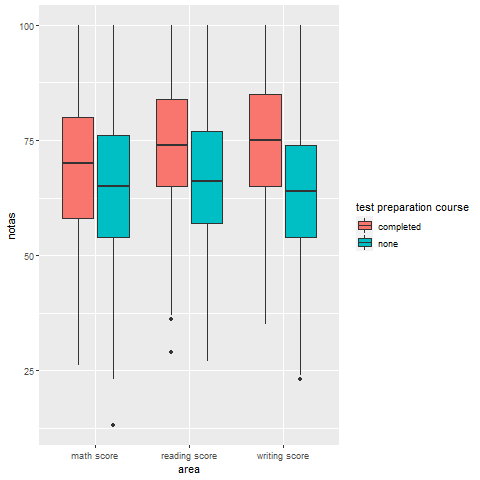
\includegraphics[width=0.6\linewidth]{plot2} \end{center}

\hypertarget{cuestiuxf3n-3.-1-punto}{%
\subsection{\texorpdfstring{Cuestión 3. \textbf{1
punto}}{Cuestión 3. 1 punto}}\label{cuestiuxf3n-3.-1-punto}}

Genera el gráfico (con \texttt{ggplot2}) e INTERPRETA el siguiente
gráfico

\begin{center}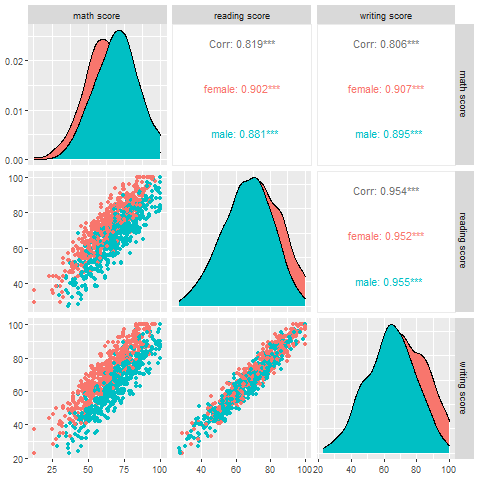
\includegraphics[width=0.6\linewidth]{plot3} \end{center}

\hypertarget{parte-2.-estaduxedstica-inferencial}{%
\section{Parte 2. Estadística
Inferencial}\label{parte-2.-estaduxedstica-inferencial}}

Nos piden analizar los datos de la
\href{http://insideairbnb.com/get-the-data.html}{web de Airbnb} para
Mallorca de septiembre de 2022 y junio de 2022 (se adjuntan) los
ficheros .

Cargad en un \texttt{dataframe} los datos del fichero
\texttt{listings.csv} (descomprimido a partir de
\texttt{listings.csv.gz}).

Vamos a cargar los datos y seleccionar algunas variables
\texttt{price,\ review\_scores\_rating} y
\texttt{neighbourhood\_cleansed}.

\begin{Shaded}
\begin{Highlighting}[]
\CommentTok{\#library(tidyverse)}
\NormalTok{data\_june}\OtherTok{=}\NormalTok{readr}\SpecialCharTok{::}\FunctionTok{read\_csv}\NormalTok{(}\StringTok{"data/listings\_mallorca\_june\_2022.csv"}\NormalTok{)}\CommentTok{\# }
\end{Highlighting}
\end{Shaded}

\begin{verbatim}
## Rows: 18298 Columns: 74
## -- Column specification --------------------------------------------------------
## Delimiter: ","
## chr  (24): listing_url, name, description, neighborhood_overview, picture_ur...
## dbl  (37): id, scrape_id, host_id, host_listings_count, host_total_listings_...
## lgl   (8): host_is_superhost, host_has_profile_pic, host_identity_verified, ...
## date  (5): last_scraped, host_since, calendar_last_scraped, first_review, la...
## 
## i Use `spec()` to retrieve the full column specification for this data.
## i Specify the column types or set `show_col_types = FALSE` to quiet this message.
\end{verbatim}

\begin{Shaded}
\begin{Highlighting}[]
\FunctionTok{print}\NormalTok{(}\FunctionTok{object.size}\NormalTok{(data\_june),}\AttributeTok{units=}\StringTok{"MB"}\NormalTok{,}\AttributeTok{stardard=}\StringTok{"SI"}\NormalTok{)}
\end{Highlighting}
\end{Shaded}

\begin{verbatim}
## 47.1 Mb
\end{verbatim}

\begin{Shaded}
\begin{Highlighting}[]
\CommentTok{\#glimpse(data\_june)}
\FunctionTok{gsub}\NormalTok{(}\AttributeTok{pattern=}\StringTok{"[}\SpecialCharTok{\textbackslash{}\textbackslash{}}\StringTok{$]|[,]"}\NormalTok{,}\AttributeTok{replacement=}\StringTok{""}\NormalTok{,data\_june}\SpecialCharTok{$}\NormalTok{price[}\DecValTok{1}\SpecialCharTok{:}\DecValTok{10}\NormalTok{])}
\end{Highlighting}
\end{Shaded}

\begin{verbatim}
##  [1] "118.00" "173.00" "120.00" "300.00" "372.00" "195.00" "237.00" "286.00"
##  [9] "135.00" "86.00"
\end{verbatim}

\begin{Shaded}
\begin{Highlighting}[]
\FunctionTok{as.numeric}\NormalTok{(}\FunctionTok{gsub}\NormalTok{(}\AttributeTok{pattern=}\StringTok{"[}\SpecialCharTok{\textbackslash{}\textbackslash{}}\StringTok{$]|[,]"}\NormalTok{,}\AttributeTok{replacement=}\StringTok{""}\NormalTok{,data\_june}\SpecialCharTok{$}\NormalTok{price[}\DecValTok{1}\SpecialCharTok{:}\DecValTok{10}\NormalTok{]))}
\end{Highlighting}
\end{Shaded}

\begin{verbatim}
##  [1] 118 173 120 300 372 195 237 286 135  86
\end{verbatim}

\begin{Shaded}
\begin{Highlighting}[]
\NormalTok{data\_june}\SpecialCharTok{$}\NormalTok{price}\OtherTok{=}\FunctionTok{as.numeric}\NormalTok{(}\FunctionTok{gsub}\NormalTok{(}\AttributeTok{pattern=}\StringTok{"[}\SpecialCharTok{\textbackslash{}\textbackslash{}}\StringTok{$]|[,]"}\NormalTok{,}\AttributeTok{replacement=}\StringTok{""}\NormalTok{,data\_june}\SpecialCharTok{$}\NormalTok{price))}
\FunctionTok{head}\NormalTok{(data\_june}\SpecialCharTok{$}\NormalTok{price)}
\end{Highlighting}
\end{Shaded}

\begin{verbatim}
## [1] 118 173 120 300 372 195
\end{verbatim}

\begin{Shaded}
\begin{Highlighting}[]
\FunctionTok{class}\NormalTok{(data\_june}\SpecialCharTok{$}\NormalTok{price)}
\end{Highlighting}
\end{Shaded}

\begin{verbatim}
## [1] "numeric"
\end{verbatim}

\begin{Shaded}
\begin{Highlighting}[]
\NormalTok{data\_june}\OtherTok{=}\NormalTok{ data\_june }\SpecialCharTok{\%\textgreater{}\%} \FunctionTok{select}\NormalTok{(price,review\_scores\_rating,neighbourhood\_cleansed)}
\FunctionTok{glimpse}\NormalTok{(data\_june)}
\end{Highlighting}
\end{Shaded}

\begin{verbatim}
## Rows: 18,298
## Columns: 3
## $ price                  <dbl> 118, 173, 120, 300, 372, 195, 237, 286, 135, 86~
## $ review_scores_rating   <dbl> 4.73, 4.17, NA, 5.00, 5.00, 4.82, 5.00, 4.90, N~
## $ neighbourhood_cleansed <chr> "Sóller", "Pollença", "Sóller", "Alcúdia", "Mur~
\end{verbatim}

\hypertarget{pregunta-1.-1-punto}{%
\subsection{\texorpdfstring{Pregunta 1. \textbf{1
punto}}{Pregunta 1. 1 punto}}\label{pregunta-1.-1-punto}}

\begin{enumerate}
\def\labelenumi{\alph{enumi}.}
\item
  Calcular una estimación puntual de la media para la variable
  \texttt{price} y el error estándar del estimador.
\item
  Calcular un intervalo de confianza, al nivel de confianza del 95\%,
  para la variable \texttt{price}.
\end{enumerate}

\hypertarget{soluciuxf3n}{%
\subsection{Solución}\label{soluciuxf3n}}

\begin{enumerate}
\def\labelenumi{\alph{enumi})}
\tightlist
\item
\end{enumerate}

\begin{Shaded}
\begin{Highlighting}[]
\NormalTok{media }\OtherTok{=} \FunctionTok{mean}\NormalTok{(data\_june}\SpecialCharTok{$}\NormalTok{price)}
\NormalTok{media}
\end{Highlighting}
\end{Shaded}

\begin{verbatim}
## [1] 286.2452
\end{verbatim}

\begin{Shaded}
\begin{Highlighting}[]
\NormalTok{n }\OtherTok{=} \FunctionTok{length}\NormalTok{(data\_june}\SpecialCharTok{$}\NormalTok{price)}
\NormalTok{error }\OtherTok{=} \FunctionTok{sd}\NormalTok{(data\_june}\SpecialCharTok{$}\NormalTok{price)}\SpecialCharTok{/}\FunctionTok{sqrt}\NormalTok{(n)}
\NormalTok{error}
\end{Highlighting}
\end{Shaded}

\begin{verbatim}
## [1] 6.333008
\end{verbatim}

\begin{enumerate}
\def\labelenumi{\alph{enumi})}
\setcounter{enumi}{1}
\tightlist
\item
\end{enumerate}

\begin{Shaded}
\begin{Highlighting}[]
\NormalTok{alpha }\OtherTok{=} \DecValTok{1}\FloatTok{{-}0.95}
\NormalTok{intconf }\OtherTok{=} \FunctionTok{c}\NormalTok{(media}\SpecialCharTok{{-}}\FunctionTok{qt}\NormalTok{(}\DecValTok{1}\SpecialCharTok{{-}}\NormalTok{(alpha}\SpecialCharTok{/}\DecValTok{2}\NormalTok{),}\AttributeTok{df=}\NormalTok{n}\DecValTok{{-}1}\NormalTok{)}\SpecialCharTok{*}\NormalTok{error,media}\SpecialCharTok{+}\FunctionTok{qt}\NormalTok{(}\DecValTok{1}\SpecialCharTok{{-}}\NormalTok{(alpha}\SpecialCharTok{/}\DecValTok{2}\NormalTok{),}\AttributeTok{df=}\NormalTok{n}\DecValTok{{-}1}\NormalTok{)}\SpecialCharTok{*}\NormalTok{error)}
\NormalTok{intconf}
\end{Highlighting}
\end{Shaded}

\begin{verbatim}
## [1] 273.8319 298.6585
\end{verbatim}

\hypertarget{pregunta-2.-2-puntos}{%
\subsection{\texorpdfstring{Pregunta 2. \textbf{2
puntos}}{Pregunta 2. 2 puntos}}\label{pregunta-2.-2-puntos}}

\begin{enumerate}
\def\labelenumi{\alph{enumi}.}
\tightlist
\item
  Supongamos que un responsable de Airbnb asegura que el porcentaje de
  los valores de \texttt{review\_scores\_rating} mayor o igual que 4.5
  es del 79.5\% . Contrastad esta hipótesis con los datos de Mallorca.
\item
  Calcular un intervalo de confianza del 95\% asociado a este contraste
  por el método exacto, el de Wilson y el Laplace.
\end{enumerate}

\hypertarget{soluciuxf3n-1}{%
\subsection{Solución}\label{soluciuxf3n-1}}

\begin{enumerate}
\def\labelenumi{\alph{enumi})}
\tightlist
\item
  Queremos contrastar la siguiente hipótesis: H0: μ = 4.5 H1: μ
  \textgreater{} 4.5
\end{enumerate}

\begin{Shaded}
\begin{Highlighting}[]
\NormalTok{n }\OtherTok{=} \FunctionTok{length}\NormalTok{(data\_june}\SpecialCharTok{$}\NormalTok{review\_scores\_rating)}
\DocumentationTok{\#\#n}
\NormalTok{media }\OtherTok{=} \FunctionTok{mean}\NormalTok{(data\_june}\SpecialCharTok{$}\NormalTok{review\_scores\_rating)}
\DocumentationTok{\#\#media}
\FunctionTok{t.test}\NormalTok{(data\_june}\SpecialCharTok{$}\NormalTok{review\_scores\_rating, }\AttributeTok{mu=}\FloatTok{4.5}\NormalTok{, }\AttributeTok{alternative=}\StringTok{"greater"}\NormalTok{, }\AttributeTok{conf.level=}\FloatTok{0.95}\NormalTok{)}
\end{Highlighting}
\end{Shaded}

\begin{verbatim}
## 
##  One Sample t-test
## 
## data:  data_june$review_scores_rating
## t = 26.817, df = 12662, p-value < 2.2e-16
## alternative hypothesis: true mean is greater than 4.5
## 95 percent confidence interval:
##  4.635406      Inf
## sample estimates:
## mean of x 
##  4.644254
\end{verbatim}

\begin{enumerate}
\def\labelenumi{\alph{enumi})}
\setcounter{enumi}{1}
\tightlist
\item
\end{enumerate}

Método exacto:

\begin{Shaded}
\begin{Highlighting}[]
\NormalTok{epitools}\SpecialCharTok{::}\FunctionTok{binom.exact}\NormalTok{(}\FunctionTok{table}\NormalTok{(data\_june}\SpecialCharTok{$}\NormalTok{review\_scores\_rating}\SpecialCharTok{\textgreater{}}\FloatTok{4.5}\NormalTok{)[}\StringTok{"TRUE"}\NormalTok{],}\FunctionTok{length}\NormalTok{(data\_june}\SpecialCharTok{$}\NormalTok{review\_scores\_rating),}\AttributeTok{conf.level =} \FloatTok{0.95}\NormalTok{)}
\end{Highlighting}
\end{Shaded}

\begin{verbatim}
##         x     n proportion     lower     upper conf.level
## TRUE 9565 18298  0.5227347 0.5154671 0.5299951       0.95
\end{verbatim}

Método Wilson:

\begin{Shaded}
\begin{Highlighting}[]
\NormalTok{epitools}\SpecialCharTok{::}\FunctionTok{binom.wilson}\NormalTok{(}\FunctionTok{table}\NormalTok{(data\_june}\SpecialCharTok{$}\NormalTok{review\_scores\_rating}\SpecialCharTok{\textgreater{}}\FloatTok{4.5}\NormalTok{)[}\StringTok{"TRUE"}\NormalTok{],}\FunctionTok{length}\NormalTok{(data\_june}\SpecialCharTok{$}\NormalTok{review\_scores\_rating),}\AttributeTok{conf.level =} \FloatTok{0.95}\NormalTok{)}
\end{Highlighting}
\end{Shaded}

\begin{verbatim}
##         x     n proportion     lower     upper conf.level
## TRUE 9565 18298  0.5227347 0.5154936 0.5299663       0.95
\end{verbatim}

Método Laplace:

\begin{Shaded}
\begin{Highlighting}[]
\NormalTok{epitools}\SpecialCharTok{::}\FunctionTok{binom.approx}\NormalTok{(}\FunctionTok{table}\NormalTok{(data\_june}\SpecialCharTok{$}\NormalTok{review\_scores\_rating}\SpecialCharTok{\textgreater{}}\FloatTok{4.5}\NormalTok{)[}\StringTok{"TRUE"}\NormalTok{],}\FunctionTok{length}\NormalTok{(data\_june}\SpecialCharTok{$}\NormalTok{review\_scores\_rating), }\AttributeTok{conf.level =} \FloatTok{0.95}\NormalTok{)}
\end{Highlighting}
\end{Shaded}

\begin{verbatim}
##         x     n proportion     lower     upper conf.level
## TRUE 9565 18298  0.5227347 0.5154976 0.5299719       0.95
\end{verbatim}

\hypertarget{pregunta-3.-2-puntos}{%
\subsection{\texorpdfstring{Pregunta 3. \textbf{2
puntos}}{Pregunta 3. 2 puntos}}\label{pregunta-3.-2-puntos}}

Considera ahora los datos de \texttt{price} para del mes junio de 2022
de las dos zonas de Mallorca con más apartamentos vacacionales

\begin{Shaded}
\begin{Highlighting}[]
\FunctionTok{sort}\NormalTok{(}\FunctionTok{table}\NormalTok{(data\_june}\SpecialCharTok{$}\NormalTok{neighbourhood\_cleansed),}\AttributeTok{decreasing =} \ConstantTok{TRUE}\NormalTok{)[}\DecValTok{1}\SpecialCharTok{:}\DecValTok{4}\NormalTok{]}
\end{Highlighting}
\end{Shaded}

\begin{verbatim}
## 
##          Pollença Palma de Mallorca           Alcúdia          Santanyí 
##              2625              1923              1897              1015
\end{verbatim}

\begin{enumerate}
\def\labelenumi{\alph{enumi}.}
\tightlist
\item
  Decidid si las varianzas del precio en las dos zonas son iguales o
  diferentes. Considera que las distribuciones de los valores de precio
  en las poblaciones son normales.
\item
  Dad un intervalo de confianza del 95\% para comparar las varianzas.
  Interpretar adecuadamente el resultado.
\end{enumerate}

\hypertarget{soluciuxf3n-2}{%
\subsection{Solución}\label{soluciuxf3n-2}}

\begin{enumerate}
\def\labelenumi{\alph{enumi})}
\tightlist
\item
  Plantearemos el siguiente contraste:
\end{enumerate}

H0: σ1 = σ2 H1: σ1 ≠ σ2

\begin{Shaded}
\begin{Highlighting}[]
\NormalTok{data\_june }\SpecialCharTok{\%\textgreater{}\%}
  \FunctionTok{filter}\NormalTok{(neighbourhood\_cleansed}\SpecialCharTok{==}\StringTok{"Palma de Mallorca"}\NormalTok{) }\SpecialCharTok{\%\textgreater{}\%}
  \FunctionTok{select}\NormalTok{(}\DecValTok{1}\NormalTok{)}
\end{Highlighting}
\end{Shaded}

\begin{verbatim}
## # A tibble: 1,923 x 1
##    price
##    <dbl>
##  1    80
##  2   171
##  3    65
##  4   110
##  5    75
##  6    65
##  7    25
##  8    46
##  9   238
## 10   120
## # ... with 1,913 more rows
\end{verbatim}

\begin{Shaded}
\begin{Highlighting}[]
\DocumentationTok{\#\#EnvStats:: varTest(palma,conf.level=0.95)$conf.int}
\end{Highlighting}
\end{Shaded}

\begin{enumerate}
\def\labelenumi{\alph{enumi})}
\setcounter{enumi}{1}
\tightlist
\item
\end{enumerate}

\hypertarget{pregunta-4.-2-puntos}{%
\subsection{\texorpdfstring{Pregunta 4. \textbf{2
puntos}}{Pregunta 4. 2 puntos}}\label{pregunta-4.-2-puntos}}

\begin{enumerate}
\def\labelenumi{\alph{enumi}.}
\tightlist
\item
  A partir de los resultados del apartado anterior contrastad la
  hipótesis de que los precios medios en las dos ciudades son iguales
  contra que son distintos.
\item
  Calcular un intervalo de confianza del 95\% para la diferencia de
  precios.
\end{enumerate}

\hypertarget{soluciuxf3n-3}{%
\subsection{Solución}\label{soluciuxf3n-3}}

\end{document}
